\section{Modèle de processeur}

Cette partie vise à présenter les modifications du processeur afin d'assembler un système complète avec les blocs \gls{RAM}. 
Pour de tester la mémoire réalisée dans la partie précédente, le sujet fourni imagine un modèle de processeur élémentaire.
Cela permet à la fois de contextualiser le miniprojet tout en faisait appel aux connaissances d'architecture des ordinateurs vue les années passées.
Un modèle de processeur appelé \texttt{simple proc} est donné aux étudiants sous forme d'un code \textit{Verilog}.
Il est composé d'une mémoire interne pour stocker les instructions et données, mais ne comporte aucune entrée sortie.
Il n'est donc pas synthétisable, mais uniquement simulable.
L'objectif est de faire les modifications nécessaires pour assurer la compatibilité avec les blocs \gls{RAM}.
Cela passe par l'ajout d'un certain nombre de signaux et par la modification de l'\gls{ISA}. \\ 
\gap

Comme indiqué dans l'introduction, le logiciel \textit{Verilator} a été utilisé pour la simulation.
Sa particularité est de transformer la description \textit{Verilog} en \textit{C++}.
Le testbench peut être écrit en \textit{C++} offrant ainsi une vue plus haut niveau apprécié pour le test.
Le projet est largement utilisé dans le monde académique comme dans l'industrie.
On peut ainsi voir RISC-V, Microchip, NXP, Intel parmi ses utilisateurs.


\subsection{Modification de l'architecture}
La première modification à apporter est l'ajout d'entrées sorties au processeur.
Cela doit permettre la connexion avec le bloc quadram.
Comme une entité (entity) en VHDL, le mot clé \texttt{module} permet d'adopter une vue externe.
On ajoute alors deux entrées clock (clk) et reset (nRst) pour la synchronisation.
Nous disposons dès lors d'une horloge, les instructions non synthétisable \texttt{step} peuvent être retirées après avoir rendu synchrone le process principal. La ligne \textit{Verilog} suivante permet cela.
\begin{lstlisting}
    always @ (posedge clk)
\end{lstlisting}
Il a été choisi précédemment de dupliquer le bus de données selon le sens de communication pour ne pas gérer la complexité induite par la bidirectionalité. Deux tableaux de bits \texttt{datain}, \texttt{dataout} sont définis un en entrée et l'autre en sortie. Leur taille est passée en paramètre pour garantir la généricité. Finalement, le bus d'adresse en déclaré en sortie car, seul le processeur en a le contrôle. Sa taille est, elle aussi, variable.
Le signal \texttt{we} pour "write enable" est utile pour contrôler la \gls{RAM} est déclarée comme sortie.
\begin{figure}[H]
    \centering
    \includegraphics[width=0.5\linewidth]{entity_proc.png}
    \caption{Entité simple proc}
    \label{entity_proc}
\end{figure}

Après la synthèse, la vue externe obtenue figure \ref{entity_proc} est bien celle attendue.
Tous les signaux définis sont présents. Les paramètres pour la longueur des bus de données et d'adresse sont respectivement 32 et 12 dans cet exemple. \\
\gap

La seconde modification est nécessaire en raison du changement de mémoire. 
Le processeur est initialement conçu avec une mémoire interne. 
La contraire concernant l'usage d'une mémoire externe rend l'accès à la donnée impossible pour les opérations arithmétiques.
Pour palier à cela, la solution est l'ajout de registres tampons d'une longueur égale à celle du bus de données.
Leur politique de gestion est explicitement laissée libre dans le sujet.
Les choix effectués par les étudiants concepteurs ne concernent pas la déclaration des registres, mais plutôt l'\gls{ISA}.
C'est pourquoi cette question sera abordée dans la partie suivante. \\
\gap

Le signal reset est choisi comme étant actif à l'état bas, son activation a pour effet de mettre à zéro les registres PC, IR, SR, reg\_A, reg\_B et le signal we.

\subsection{Modification de l'ISA}
%TODO Définir l'ISA
Une solution a été implémentée pour palier à l'inaccessibilité des données par les instructions arithmétiques.
Elle vise à ajouter deux registres tampons A et B.
Il existe différentes philosophies de processeur parmi elles les plus connues, \gls{RISC} et \gls{CISC}.
Elles sont différentes sur plusieurs points. Pour ce qui nous intéresse ici, les architecture \gls{RISC} sont plus simple et exécute les instructions en un seul coup d'horloge. Les processeurs \gls{CISC} sont plus complexes et disposent d'instructions plus puissantes. Étudions cela à travers l'addition.
% montrer que CISC prermet l'addition de case mémoire quand RISC a besoin de deux LD.
% Ajouter les sources
Pour des questions de simplicité, mais aussi car l'architecture \gls{RISC} sont particulièrement intéressante pour l'embarqué comme le montre la popularité de ARM et RISC-V \textbf{nous choisirons la philosophie \gls{RISC}}.

Il convient alors de modifier les instructions arithmétiques. 
La règle générale est alors $A = A o B$ ou les lettres A et B représentent les registres et le symbole $o$ les opérations arithmétiques telles que l'addition, la soustraction et la multiplication. Le résultat du complément est également stocké dans A. 
Le code \textit{Verilog} dans le cas de l'addition est le suivant :
\begin{lstlisting}
`ADD:
begin
    reg_A = reg_A + reg_B;
    setcondcode(reg_A);
end
\end{lstlisting}
L'appel à la fonction \texttt{setcondcode()} met à jour l'état du registre SR avec le résultat du calcul. \\
\gap

Dans l'état actuel du processeur, il n'est pas possible d'affecter une valeur aux registres A et B.
Pour palier à cela, deux instructions "load" sont ajoutées LDA et LDB.
Il existe une subtilité quant à leur mise en place. Contrairement à la mémoire interne, la RAM n'est pas accessible immédiatement. 
D'abord l'adresse est placée sur le bus puis, un instant après, la valeur de la case mémoire est placée sur le bus de données.
Cela écarte une solution naïve qui viserait à écrire l'adresse et récolter la donnée de manière synchrone à l'horloge.
Il faudrait plutôt, affecter la valeur du bus au registre durant toute l'instruction et ne la sauvegarder qu'à la fin.
La solution que nous proposons est l'ajout d'un signal \texttt{write\_A} qui sera valide toute la durée de l'instruction LDA.
Ce dernier est placé dans la liste de sensibilité d'un second process, asynchrone cette fois, autorise l'écriture dans le registre. 
Le code de ce process est le suivant :
\begin{lstlisting}
always @(write_A)
begin
  if(write_A)
    reg_A <= datain;
end
\end{lstlisting}
Le registre prend pour valeur l'état du bus de données pendant toute la durée du cycle horloge et conserve la dernière.
La mémoire doit fournir la donnée avant la fin du cycle (on néglige les temps de maintien) ce qui semble être une contrainte acceptable.
La solution est dupliquée pour le registre B.
\begin{figure}[H]
    \centering
    \includegraphics[width=0.8\linewidth]{chrono_mem_delay_solved_cmd.draw.png}
    \caption{Chronogramme test LDA et LDB}
    \label{fig:test_LD}
\end{figure}
Le chronogramme commenté figure \ref{fig:test_LD} présente les résultats obtenus après simulation.
Un testbench permet de charger la mémoire avec les instructions \texttt{LDA 0x78} et \texttt{LDB 0x91}. 
Il fournit ensuite une réponse semblable au comportement de la \gls{RAM} en plaçant après un délai une valeur sur le bus de donnée.
Pour des raisons de facilité d'écriture du testbench la valeur est donnée synchrone au front descendant.
Cela n'est pas nécessaire au bon fonctionnement du processeur.
A l'instant du label 1, l'instruction \texttt{LDA 0x78} est exécutée et 0x78 est placé sur le bus d'adresse et \texttt{write\_A} passe à l'état haut.
Puis à l'instant 2, la donnée 0x19 est fournie et immédiatement affectée au registre.
Enfin, à l'instant 3, la valeur 0x19 est maintenue dans le registre. 
L'instruction de chargement (load) a fonctionné.
Le même raisonnement s'applique pour \texttt{LDB}.


%Nous n'avons pas réussi à définir le codage des instructions de manière générique dans le temps imparti.
